\documentclass[twoside]{book}

% Packages required by doxygen
\usepackage{fixltx2e}
\usepackage{calc}
\usepackage{doxygen}
\usepackage[export]{adjustbox} % also loads graphicx
\usepackage{graphicx}
\usepackage[utf8]{inputenc}
\usepackage{makeidx}
\usepackage{multicol}
\usepackage{multirow}
\PassOptionsToPackage{warn}{textcomp}
\usepackage{textcomp}
\usepackage[nointegrals]{wasysym}
\usepackage[table]{xcolor}

% Font selection
\usepackage[T1]{fontenc}
\usepackage[scaled=.90]{helvet}
\usepackage{courier}
\usepackage{amssymb}
\usepackage{sectsty}
\renewcommand{\familydefault}{\sfdefault}
\allsectionsfont{%
  \fontseries{bc}\selectfont%
  \color{darkgray}%
}
\renewcommand{\DoxyLabelFont}{%
  \fontseries{bc}\selectfont%
  \color{darkgray}%
}
\newcommand{\+}{\discretionary{\mbox{\scriptsize$\hookleftarrow$}}{}{}}

% Page & text layout
\usepackage{geometry}
\geometry{%
  a4paper,%
  top=2.5cm,%
  bottom=2.5cm,%
  left=2.5cm,%
  right=2.5cm%
}
\tolerance=750
\hfuzz=15pt
\hbadness=750
\setlength{\emergencystretch}{15pt}
\setlength{\parindent}{0cm}
\setlength{\parskip}{3ex plus 2ex minus 2ex}
\makeatletter
\renewcommand{\paragraph}{%
  \@startsection{paragraph}{4}{0ex}{-1.0ex}{1.0ex}{%
    \normalfont\normalsize\bfseries\SS@parafont%
  }%
}
\renewcommand{\subparagraph}{%
  \@startsection{subparagraph}{5}{0ex}{-1.0ex}{1.0ex}{%
    \normalfont\normalsize\bfseries\SS@subparafont%
  }%
}
\makeatother

% Headers & footers
\usepackage{fancyhdr}
\pagestyle{fancyplain}
\fancyhead[LE]{\fancyplain{}{\bfseries\thepage}}
\fancyhead[CE]{\fancyplain{}{}}
\fancyhead[RE]{\fancyplain{}{\bfseries\leftmark}}
\fancyhead[LO]{\fancyplain{}{\bfseries\rightmark}}
\fancyhead[CO]{\fancyplain{}{}}
\fancyhead[RO]{\fancyplain{}{\bfseries\thepage}}
\fancyfoot[LE]{\fancyplain{}{}}
\fancyfoot[CE]{\fancyplain{}{}}
\fancyfoot[RE]{\fancyplain{}{\bfseries\scriptsize Generated by Doxygen }}
\fancyfoot[LO]{\fancyplain{}{\bfseries\scriptsize Generated by Doxygen }}
\fancyfoot[CO]{\fancyplain{}{}}
\fancyfoot[RO]{\fancyplain{}{}}
\renewcommand{\footrulewidth}{0.4pt}
\renewcommand{\chaptermark}[1]{%
  \markboth{#1}{}%
}
\renewcommand{\sectionmark}[1]{%
  \markright{\thesection\ #1}%
}

% Indices & bibliography
\usepackage{natbib}
\usepackage[titles]{tocloft}
\setcounter{tocdepth}{3}
\setcounter{secnumdepth}{5}
\makeindex

% Hyperlinks (required, but should be loaded last)
\usepackage{ifpdf}
\ifpdf
  \usepackage[pdftex,pagebackref=true]{hyperref}
\else
  \usepackage[ps2pdf,pagebackref=true]{hyperref}
\fi
\hypersetup{%
  colorlinks=true,%
  linkcolor=blue,%
  citecolor=blue,%
  unicode%
}

% Custom commands
\newcommand{\clearemptydoublepage}{%
  \newpage{\pagestyle{empty}\cleardoublepage}%
}

\usepackage{caption}
\captionsetup{labelsep=space,justification=centering,font={bf},singlelinecheck=off,skip=4pt,position=top}

%===== C O N T E N T S =====

\begin{document}

% Titlepage & ToC
\hypersetup{pageanchor=false,
             bookmarksnumbered=true,
             pdfencoding=unicode
            }
\pagenumbering{alph}
\begin{titlepage}
\vspace*{7cm}
\begin{center}%
{\Large My Project }\\
\vspace*{1cm}
{\large Generated by Doxygen 1.8.13}\\
\end{center}
\end{titlepage}
\clearemptydoublepage
\pagenumbering{roman}
\tableofcontents
\clearemptydoublepage
\pagenumbering{arabic}
\hypersetup{pageanchor=true}

%--- Begin generated contents ---
\chapter{Hierarchical Index}
\section{Class Hierarchy}
This inheritance list is sorted roughly, but not completely, alphabetically\+:\begin{DoxyCompactList}
\item \contentsline{section}{Bounding\+Box}{\pageref{classBoundingBox}}{}
\item \contentsline{section}{Game\+Asset}{\pageref{classGameAsset}}{}
\begin{DoxyCompactList}
\item \contentsline{section}{Camera}{\pageref{classCamera}}{}
\item \contentsline{section}{Cube\+Asset}{\pageref{classCubeAsset}}{}
\end{DoxyCompactList}
\item \contentsline{section}{Game\+Asset\+Manager}{\pageref{classGameAssetManager}}{}
\item \contentsline{section}{Game\+World}{\pageref{classGameWorld}}{}
\item \contentsline{section}{Point3}{\pageref{classPoint3}}{}
\item \contentsline{section}{S\+D\+L\+Window\+Deleter}{\pageref{structSDLWindowDeleter}}{}
\item Test\+Case\begin{DoxyCompactList}
\item \contentsline{section}{Test\+Bounding\+Box}{\pageref{classTestBoundingBox}}{}
\end{DoxyCompactList}
\item \contentsline{section}{Vector3}{\pageref{classVector3}}{}
\end{DoxyCompactList}

\chapter{Class Index}
\section{Class List}
Here are the classes, structs, unions and interfaces with brief descriptions\+:\begin{DoxyCompactList}
\item\contentsline{section}{\hyperlink{classBoundingBox}{Bounding\+Box} }{\pageref{classBoundingBox}}{}
\item\contentsline{section}{\hyperlink{classCamera}{Camera} }{\pageref{classCamera}}{}
\item\contentsline{section}{\hyperlink{classCubeAsset}{Cube\+Asset} }{\pageref{classCubeAsset}}{}
\item\contentsline{section}{\hyperlink{classGameAsset}{Game\+Asset} }{\pageref{classGameAsset}}{}
\item\contentsline{section}{\hyperlink{classGameAssetManager}{Game\+Asset\+Manager} }{\pageref{classGameAssetManager}}{}
\item\contentsline{section}{\hyperlink{classGameWorld}{Game\+World} }{\pageref{classGameWorld}}{}
\item\contentsline{section}{\hyperlink{classPoint3}{Point3} }{\pageref{classPoint3}}{}
\item\contentsline{section}{\hyperlink{structSDLWindowDeleter}{S\+D\+L\+Window\+Deleter} }{\pageref{structSDLWindowDeleter}}{}
\item\contentsline{section}{\hyperlink{classTestBoundingBox}{Test\+Bounding\+Box} }{\pageref{classTestBoundingBox}}{}
\item\contentsline{section}{\hyperlink{classVector3}{Vector3} }{\pageref{classVector3}}{}
\end{DoxyCompactList}

\chapter{Class Documentation}
\hypertarget{classBoundingBox}{}\section{Bounding\+Box Class Reference}
\label{classBoundingBox}\index{Bounding\+Box@{Bounding\+Box}}
\subsection*{Public Member Functions}
\begin{DoxyCompactItemize}
\item 
\mbox{\Hypertarget{classBoundingBox_a150ee0e10ba3ebf104a75cb75ec8325c}\label{classBoundingBox_a150ee0e10ba3ebf104a75cb75ec8325c}} 
{\bfseries Bounding\+Box} (const \hyperlink{classVector3}{Vector3}, const float, const float, const float)
\item 
\mbox{\Hypertarget{classBoundingBox_a36b903eded5b5650c7486ae6a9364ac6}\label{classBoundingBox_a36b903eded5b5650c7486ae6a9364ac6}} 
void {\bfseries Set\+Centre} (\hyperlink{classVector3}{Vector3} \&)
\item 
\mbox{\Hypertarget{classBoundingBox_a3a08436b44b078caab8d99eb89124a9a}\label{classBoundingBox_a3a08436b44b078caab8d99eb89124a9a}} 
bool {\bfseries Collides\+With} (const shared\+\_\+ptr$<$ \hyperlink{classBoundingBox}{Bounding\+Box} $>$)
\end{DoxyCompactItemize}
\subsection*{Friends}
\begin{DoxyCompactItemize}
\item 
\mbox{\Hypertarget{classBoundingBox_aac419ea220c5b99491665a2ae5e035f2}\label{classBoundingBox_aac419ea220c5b99491665a2ae5e035f2}} 
ostream \& {\bfseries operator$<$$<$} (ostream \&, const \hyperlink{classBoundingBox}{Bounding\+Box} \&)
\end{DoxyCompactItemize}


The documentation for this class was generated from the following files\+:\begin{DoxyCompactItemize}
\item 
Bounding\+Box.\+h\item 
Bounding\+Box.\+cc\end{DoxyCompactItemize}

\hypertarget{classCamera}{}\section{Camera Class Reference}
\label{classCamera}\index{Camera@{Camera}}
Inheritance diagram for Camera\+:\begin{figure}[H]
\begin{center}
\leavevmode
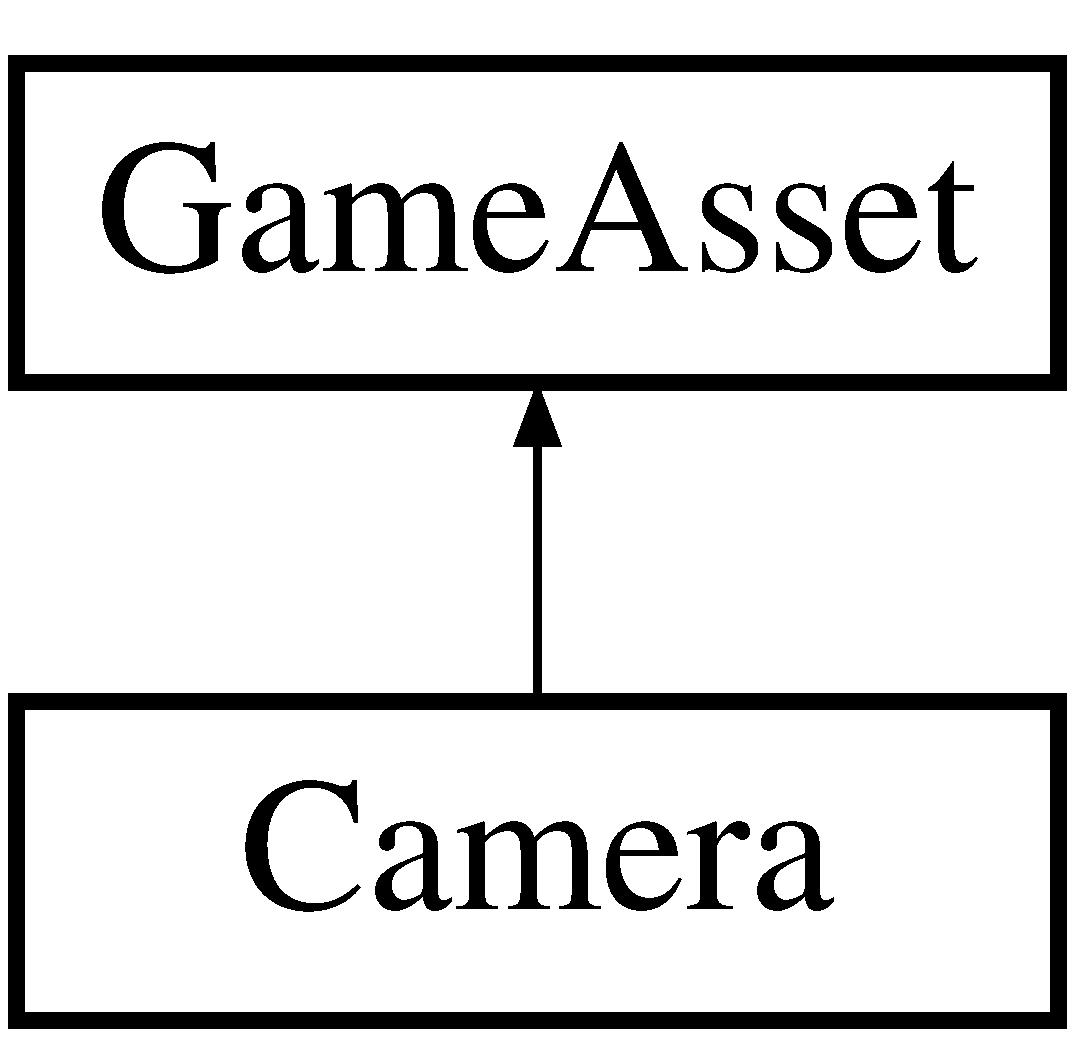
\includegraphics[height=2.000000cm]{classCamera}
\end{center}
\end{figure}
\subsection*{Public Member Functions}
\begin{DoxyCompactItemize}
\item 
\mbox{\Hypertarget{classCamera_a5569ca5967e01d3344fbf6aba36d9820}\label{classCamera_a5569ca5967e01d3344fbf6aba36d9820}} 
glm\+::mat4 {\bfseries get\+View\+Matrix} ()
\item 
\mbox{\Hypertarget{classCamera_ac147942fad5ba70bd9a7d3960258f0f5}\label{classCamera_ac147942fad5ba70bd9a7d3960258f0f5}} 
void {\bfseries move\+\_\+\+PositiveY} (float)
\item 
\mbox{\Hypertarget{classCamera_a9d92e451804ad72d049bb8b2d373064d}\label{classCamera_a9d92e451804ad72d049bb8b2d373064d}} 
void {\bfseries move\+\_\+\+NegativeY} (float)
\item 
\mbox{\Hypertarget{classCamera_a9075c40ce6f42f8e1ebbe82302537a5f}\label{classCamera_a9075c40ce6f42f8e1ebbe82302537a5f}} 
void {\bfseries move\+\_\+\+PositiveX} (float)
\item 
\mbox{\Hypertarget{classCamera_ac6580bfbbc54659b2985715a9da4d814}\label{classCamera_ac6580bfbbc54659b2985715a9da4d814}} 
void {\bfseries move\+\_\+\+NegativeX} (float)
\item 
\mbox{\Hypertarget{classCamera_a7e459e7241931372794d4ec981c89d8b}\label{classCamera_a7e459e7241931372794d4ec981c89d8b}} 
void {\bfseries move\+\_\+\+PositiveZ} (float)
\item 
\mbox{\Hypertarget{classCamera_abbbd13815d534f0c49ff3b9831a1a6e0}\label{classCamera_abbbd13815d534f0c49ff3b9831a1a6e0}} 
void {\bfseries move\+\_\+\+NegativeZ} (float)
\item 
\mbox{\Hypertarget{classCamera_a81a437bea2feaf9754918480fb6b90e7}\label{classCamera_a81a437bea2feaf9754918480fb6b90e7}} 
void {\bfseries Draw} (G\+Luint)
\item 
\mbox{\Hypertarget{classCamera_ad7e8f779ab27268fe301c3e4db4187a5}\label{classCamera_ad7e8f779ab27268fe301c3e4db4187a5}} 
void {\bfseries reset\+View} ()
\end{DoxyCompactItemize}
\subsection*{Public Attributes}
\begin{DoxyCompactItemize}
\item 
\mbox{\Hypertarget{classCamera_add93fedd6b9a6a6e2c784aeda624de83}\label{classCamera_add93fedd6b9a6a6e2c784aeda624de83}} 
glm\+::mat4 {\bfseries view}
\end{DoxyCompactItemize}


The documentation for this class was generated from the following files\+:\begin{DoxyCompactItemize}
\item 
Camera.\+h\item 
Camera.\+cc\end{DoxyCompactItemize}

\hypertarget{classCubeAsset}{}\section{Cube\+Asset Class Reference}
\label{classCubeAsset}\index{Cube\+Asset@{Cube\+Asset}}
Inheritance diagram for Cube\+Asset\+:\begin{figure}[H]
\begin{center}
\leavevmode
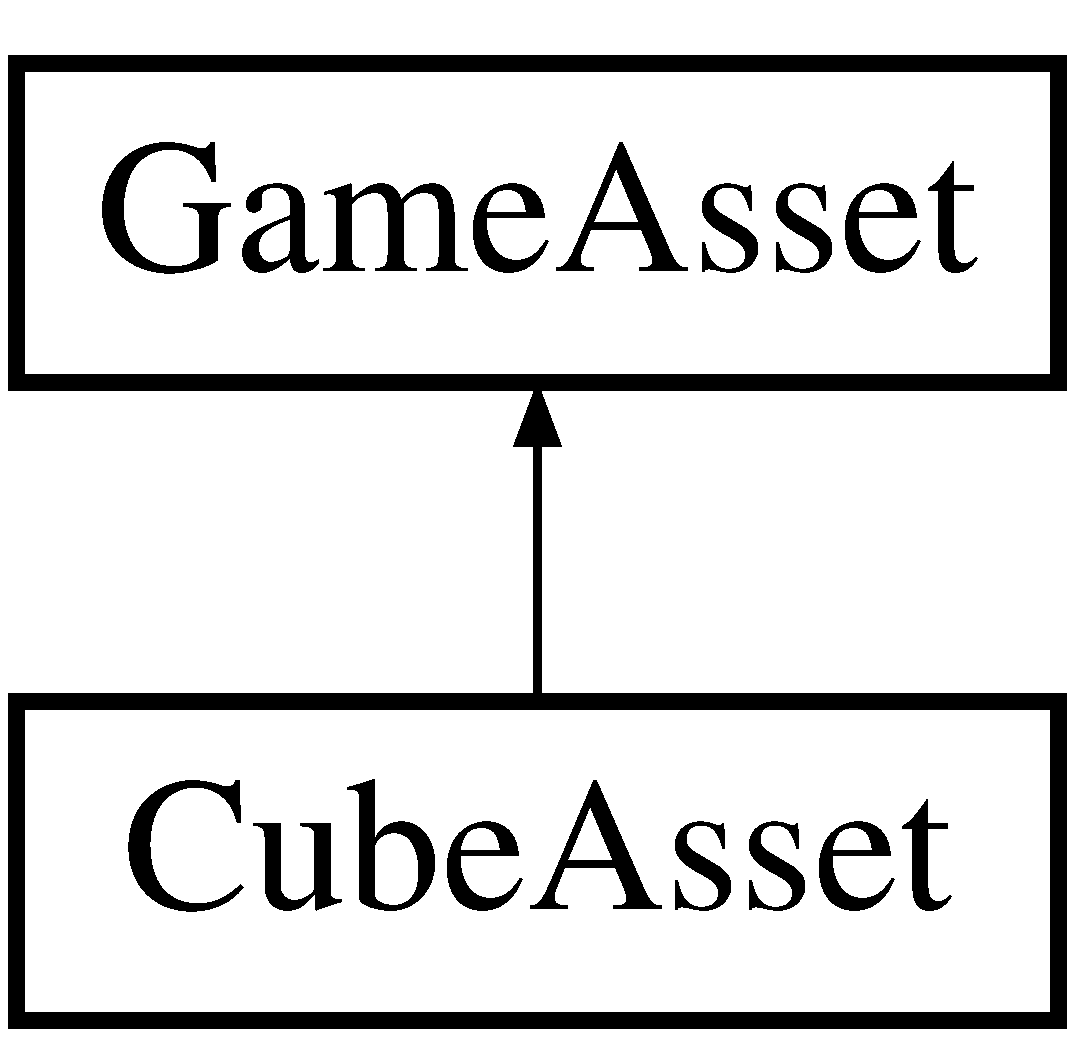
\includegraphics[height=2.000000cm]{classCubeAsset}
\end{center}
\end{figure}
\subsection*{Public Member Functions}
\begin{DoxyCompactItemize}
\item 
\mbox{\Hypertarget{classCubeAsset_a1af568486056e254ffcf98fd99947bfe}\label{classCubeAsset_a1af568486056e254ffcf98fd99947bfe}} 
virtual void {\bfseries Draw} (G\+Luint)
\end{DoxyCompactItemize}


The documentation for this class was generated from the following files\+:\begin{DoxyCompactItemize}
\item 
Cube\+Asset.\+h\item 
Cube\+Asset.\+cc\end{DoxyCompactItemize}

\hypertarget{classGameAsset}{}\section{Game\+Asset Class Reference}
\label{classGameAsset}\index{Game\+Asset@{Game\+Asset}}
Inheritance diagram for Game\+Asset\+:\begin{figure}[H]
\begin{center}
\leavevmode
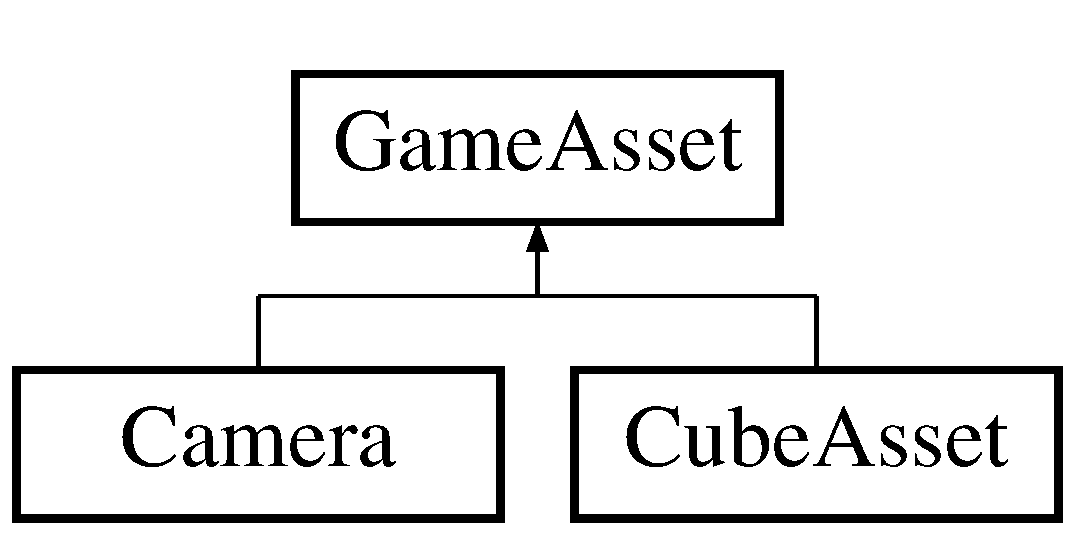
\includegraphics[height=2.000000cm]{classGameAsset}
\end{center}
\end{figure}
\subsection*{Public Member Functions}
\begin{DoxyCompactItemize}
\item 
\mbox{\Hypertarget{classGameAsset_a961aa51ca0a9961fc584c0b5d5431300}\label{classGameAsset_a961aa51ca0a9961fc584c0b5d5431300}} 
virtual void {\bfseries Draw} (G\+Luint)=0
\end{DoxyCompactItemize}


The documentation for this class was generated from the following file\+:\begin{DoxyCompactItemize}
\item 
Game\+Asset.\+h\end{DoxyCompactItemize}

\hypertarget{classGameAssetManager}{}\section{Game\+Asset\+Manager Class Reference}
\label{classGameAssetManager}\index{Game\+Asset\+Manager@{Game\+Asset\+Manager}}


{\ttfamily \#include $<$Game\+Asset\+Manager.\+h$>$}

\subsection*{Public Member Functions}
\begin{DoxyCompactItemize}
\item 
\hyperlink{classGameAssetManager_aaa0d58e276cc10ad91a7457085598a71}{Game\+Asset\+Manager} (Application\+Mode)
\item 
virtual \hyperlink{classGameAssetManager_a1270bd61ecbcca563f079803e40c9b77}{$\sim$\+Game\+Asset\+Manager} ()
\item 
\hyperlink{classGameAssetManager_a2c9adcb72faa154c87eadc9bafe5269d}{Game\+Asset\+Manager} (\hyperlink{classGameAssetManager}{Game\+Asset\+Manager} const \&)
\item 
\hyperlink{classGameAssetManager_a44f6e2fd6b8ff1dd64e5697f1be7386d}{Game\+Asset\+Manager} (\hyperlink{classGameAssetManager}{Game\+Asset\+Manager} const \&\&)
\item 
void \hyperlink{classGameAssetManager_ac72678a4ad5378c685aa6bae84a4e712}{operator=} (\hyperlink{classGameAssetManager}{Game\+Asset\+Manager} const \&)
\item 
void \hyperlink{classGameAssetManager_ad3de8ff00d55ba04728b1de8213b2349}{Add\+Asset} (std\+::shared\+\_\+ptr$<$ \hyperlink{classGameAsset}{Game\+Asset} $>$)
\item 
void \hyperlink{classGameAssetManager_a32837132bd70a9a9ed537323c2d3d886}{Draw} ()
\end{DoxyCompactItemize}


\subsection{Detailed Description}
\hyperlink{classGameAssetManager}{Game\+Asset\+Manager} is a container for Game\+Assets. It also provides utility functions to to create a simple Open\+GL program that can be used to draw a simple \hyperlink{classGameAsset}{Game\+Asset}. 

\subsection{Constructor \& Destructor Documentation}
\mbox{\Hypertarget{classGameAssetManager_aaa0d58e276cc10ad91a7457085598a71}\label{classGameAssetManager_aaa0d58e276cc10ad91a7457085598a71}} 
\index{Game\+Asset\+Manager@{Game\+Asset\+Manager}!Game\+Asset\+Manager@{Game\+Asset\+Manager}}
\index{Game\+Asset\+Manager@{Game\+Asset\+Manager}!Game\+Asset\+Manager@{Game\+Asset\+Manager}}
\subsubsection{\texorpdfstring{Game\+Asset\+Manager()}{GameAssetManager()}\hspace{0.1cm}{\footnotesize\ttfamily [1/3]}}
{\footnotesize\ttfamily Game\+Asset\+Manager\+::\+Game\+Asset\+Manager (\begin{DoxyParamCaption}\item[{Application\+Mode}]{mode }\end{DoxyParamCaption})\hspace{0.3cm}{\ttfamily [explicit]}}

Creates a \hyperlink{classGameAssetManager}{Game\+Asset\+Manager} to load the correct shaders based on the Application\+Mode. \mbox{\Hypertarget{classGameAssetManager_a1270bd61ecbcca563f079803e40c9b77}\label{classGameAssetManager_a1270bd61ecbcca563f079803e40c9b77}} 
\index{Game\+Asset\+Manager@{Game\+Asset\+Manager}!````~Game\+Asset\+Manager@{$\sim$\+Game\+Asset\+Manager}}
\index{````~Game\+Asset\+Manager@{$\sim$\+Game\+Asset\+Manager}!Game\+Asset\+Manager@{Game\+Asset\+Manager}}
\subsubsection{\texorpdfstring{$\sim$\+Game\+Asset\+Manager()}{~GameAssetManager()}}
{\footnotesize\ttfamily Game\+Asset\+Manager\+::$\sim$\+Game\+Asset\+Manager (\begin{DoxyParamCaption}{ }\end{DoxyParamCaption})\hspace{0.3cm}{\ttfamily [virtual]}}

Deletes a \hyperlink{classGameAssetManager}{Game\+Asset\+Manager}, in particular it will clean up any modifications to the Open\+GL state. \mbox{\Hypertarget{classGameAssetManager_a2c9adcb72faa154c87eadc9bafe5269d}\label{classGameAssetManager_a2c9adcb72faa154c87eadc9bafe5269d}} 
\index{Game\+Asset\+Manager@{Game\+Asset\+Manager}!Game\+Asset\+Manager@{Game\+Asset\+Manager}}
\index{Game\+Asset\+Manager@{Game\+Asset\+Manager}!Game\+Asset\+Manager@{Game\+Asset\+Manager}}
\subsubsection{\texorpdfstring{Game\+Asset\+Manager()}{GameAssetManager()}\hspace{0.1cm}{\footnotesize\ttfamily [2/3]}}
{\footnotesize\ttfamily Game\+Asset\+Manager\+::\+Game\+Asset\+Manager (\begin{DoxyParamCaption}\item[{\hyperlink{classGameAssetManager}{Game\+Asset\+Manager} const \&}]{the\+\_\+manager }\end{DoxyParamCaption})}

Unimplemented copy constructor -- this means that the \hyperlink{classGameAssetManager}{Game\+Asset\+Manager} may not work as you\textquotesingle{}d expect when being copied. \mbox{\Hypertarget{classGameAssetManager_a44f6e2fd6b8ff1dd64e5697f1be7386d}\label{classGameAssetManager_a44f6e2fd6b8ff1dd64e5697f1be7386d}} 
\index{Game\+Asset\+Manager@{Game\+Asset\+Manager}!Game\+Asset\+Manager@{Game\+Asset\+Manager}}
\index{Game\+Asset\+Manager@{Game\+Asset\+Manager}!Game\+Asset\+Manager@{Game\+Asset\+Manager}}
\subsubsection{\texorpdfstring{Game\+Asset\+Manager()}{GameAssetManager()}\hspace{0.1cm}{\footnotesize\ttfamily [3/3]}}
{\footnotesize\ttfamily Game\+Asset\+Manager\+::\+Game\+Asset\+Manager (\begin{DoxyParamCaption}\item[{\hyperlink{classGameAssetManager}{Game\+Asset\+Manager} const \&\&}]{the\+\_\+manager }\end{DoxyParamCaption})}

Unimplemented move constructor -- this unimplemented method violates the C++11 move semantics for \hyperlink{classGameAssetManager}{Game\+Asset\+Manager}. 

\subsection{Member Function Documentation}
\mbox{\Hypertarget{classGameAssetManager_ad3de8ff00d55ba04728b1de8213b2349}\label{classGameAssetManager_ad3de8ff00d55ba04728b1de8213b2349}} 
\index{Game\+Asset\+Manager@{Game\+Asset\+Manager}!Add\+Asset@{Add\+Asset}}
\index{Add\+Asset@{Add\+Asset}!Game\+Asset\+Manager@{Game\+Asset\+Manager}}
\subsubsection{\texorpdfstring{Add\+Asset()}{AddAsset()}}
{\footnotesize\ttfamily void Game\+Asset\+Manager\+::\+Add\+Asset (\begin{DoxyParamCaption}\item[{std\+::shared\+\_\+ptr$<$ \hyperlink{classGameAsset}{Game\+Asset} $>$}]{the\+\_\+asset }\end{DoxyParamCaption})}

Adds a \hyperlink{classGameAsset}{Game\+Asset} to the scene graph. \mbox{\Hypertarget{classGameAssetManager_a32837132bd70a9a9ed537323c2d3d886}\label{classGameAssetManager_a32837132bd70a9a9ed537323c2d3d886}} 
\index{Game\+Asset\+Manager@{Game\+Asset\+Manager}!Draw@{Draw}}
\index{Draw@{Draw}!Game\+Asset\+Manager@{Game\+Asset\+Manager}}
\subsubsection{\texorpdfstring{Draw()}{Draw()}}
{\footnotesize\ttfamily void Game\+Asset\+Manager\+::\+Draw (\begin{DoxyParamCaption}{ }\end{DoxyParamCaption})}

Draws each \hyperlink{classGameAsset}{Game\+Asset} in the scene graph. \mbox{\Hypertarget{classGameAssetManager_ac72678a4ad5378c685aa6bae84a4e712}\label{classGameAssetManager_ac72678a4ad5378c685aa6bae84a4e712}} 
\index{Game\+Asset\+Manager@{Game\+Asset\+Manager}!operator=@{operator=}}
\index{operator=@{operator=}!Game\+Asset\+Manager@{Game\+Asset\+Manager}}
\subsubsection{\texorpdfstring{operator=()}{operator=()}}
{\footnotesize\ttfamily void Game\+Asset\+Manager\+::operator= (\begin{DoxyParamCaption}\item[{\hyperlink{classGameAssetManager}{Game\+Asset\+Manager} const \&}]{the\+\_\+manager }\end{DoxyParamCaption})}

Unimplemented assisgnment operator -- violates the expected semantics for assignment in C++11. 

The documentation for this class was generated from the following files\+:\begin{DoxyCompactItemize}
\item 
Game\+Asset\+Manager.\+h\item 
Game\+Asset\+Manager.\+cc\end{DoxyCompactItemize}

\hypertarget{classGameWorld}{}\section{Game\+World Class Reference}
\label{classGameWorld}\index{Game\+World@{Game\+World}}


{\ttfamily \#include $<$Game\+World.\+h$>$}

\subsection*{Public Member Functions}
\begin{DoxyCompactItemize}
\item 
\hyperlink{classGameWorld_a17a84e57a80600961088afc753036f89}{Game\+World} (Application\+Mode)
\item 
void \hyperlink{classGameWorld_a275418607d8286979b276f165ad5876b}{Draw} ()
\end{DoxyCompactItemize}


\subsection{Detailed Description}
\hyperlink{classGameWorld}{Game\+World} allows us to separate the management of the game world from the nuts and bolts of game loop initialisation. The \hyperlink{classGameWorld}{Game\+World} currently has a very simplified scene graph consisiting of a single \hyperlink{classGameAssetManager}{Game\+Asset\+Manager}. 

\subsection{Constructor \& Destructor Documentation}
\mbox{\Hypertarget{classGameWorld_a17a84e57a80600961088afc753036f89}\label{classGameWorld_a17a84e57a80600961088afc753036f89}} 
\index{Game\+World@{Game\+World}!Game\+World@{Game\+World}}
\index{Game\+World@{Game\+World}!Game\+World@{Game\+World}}
\subsubsection{\texorpdfstring{Game\+World()}{GameWorld()}}
{\footnotesize\ttfamily Game\+World\+::\+Game\+World (\begin{DoxyParamCaption}\item[{Application\+Mode}]{mode }\end{DoxyParamCaption})}

We thread the Application\+Mode through the \hyperlink{classGameWorld}{Game\+World} ss we want to read it in from the user. Threading the state through the various function calls is preferable (in this case) to having some kind of global state. 

\subsection{Member Function Documentation}
\mbox{\Hypertarget{classGameWorld_a275418607d8286979b276f165ad5876b}\label{classGameWorld_a275418607d8286979b276f165ad5876b}} 
\index{Game\+World@{Game\+World}!Draw@{Draw}}
\index{Draw@{Draw}!Game\+World@{Game\+World}}
\subsubsection{\texorpdfstring{Draw()}{Draw()}}
{\footnotesize\ttfamily void Game\+World\+::\+Draw (\begin{DoxyParamCaption}{ }\end{DoxyParamCaption})}

Calling \hyperlink{classGameWorld_a275418607d8286979b276f165ad5876b}{Draw()} will draw the entire world. 

The documentation for this class was generated from the following files\+:\begin{DoxyCompactItemize}
\item 
Game\+World.\+h\item 
Game\+World.\+cc\end{DoxyCompactItemize}

\hypertarget{classPoint3}{}\section{Point3 Class Reference}
\label{classPoint3}\index{Point3@{Point3}}


{\ttfamily \#include $<$Math.\+h$>$}

\subsection*{Public Member Functions}
\begin{DoxyCompactItemize}
\item 
\mbox{\Hypertarget{classPoint3_ad0f631c28710bdde931c011074a2a68d}\label{classPoint3_ad0f631c28710bdde931c011074a2a68d}} 
{\bfseries Point3} (const float, const float, const float)
\item 
\mbox{\Hypertarget{classPoint3_aac865c72759af4a8f3001c30396e2e6f}\label{classPoint3_aac865c72759af4a8f3001c30396e2e6f}} 
{\bfseries Point3} (const \hyperlink{classVector3}{Vector3} \&)
\item 
\mbox{\Hypertarget{classPoint3_a626b55d57f4fe011906e0396f4d8cb49}\label{classPoint3_a626b55d57f4fe011906e0396f4d8cb49}} 
{\bfseries Point3} (const \hyperlink{classPoint3}{Point3} \&)
\item 
\mbox{\Hypertarget{classPoint3_a50294e5bc4bc610080f3579d35585c01}\label{classPoint3_a50294e5bc4bc610080f3579d35585c01}} 
const float {\bfseries getX} () const
\item 
\mbox{\Hypertarget{classPoint3_a692237abe7082a313a9fb92c5b7fd0a0}\label{classPoint3_a692237abe7082a313a9fb92c5b7fd0a0}} 
const float {\bfseries getY} () const
\item 
\mbox{\Hypertarget{classPoint3_a65dacc34c8c27fbef332a1dd77bde119}\label{classPoint3_a65dacc34c8c27fbef332a1dd77bde119}} 
const float {\bfseries getZ} () const
\end{DoxyCompactItemize}


\subsection{Detailed Description}
A Point representation somewhat in the style of the I\+B\+M/\+Sony Vectormath library. 

The documentation for this class was generated from the following file\+:\begin{DoxyCompactItemize}
\item 
Math.\+h\end{DoxyCompactItemize}

\hypertarget{structSDLWindowDeleter}{}\section{S\+D\+L\+Window\+Deleter Struct Reference}
\label{structSDLWindowDeleter}\index{S\+D\+L\+Window\+Deleter@{S\+D\+L\+Window\+Deleter}}
\subsection*{Public Member Functions}
\begin{DoxyCompactItemize}
\item 
\mbox{\Hypertarget{structSDLWindowDeleter_a2aedcc99c3756ae090c38badabeb10b1}\label{structSDLWindowDeleter_a2aedcc99c3756ae090c38badabeb10b1}} 
void {\bfseries operator()} (S\+D\+L\+\_\+\+Window $\ast$window)
\end{DoxyCompactItemize}


The documentation for this struct was generated from the following file\+:\begin{DoxyCompactItemize}
\item 
main.\+cc\end{DoxyCompactItemize}

\hypertarget{classTestBoundingBox}{}\section{Test\+Bounding\+Box Class Reference}
\label{classTestBoundingBox}\index{Test\+Bounding\+Box@{Test\+Bounding\+Box}}
Inheritance diagram for Test\+Bounding\+Box\+:\begin{figure}[H]
\begin{center}
\leavevmode
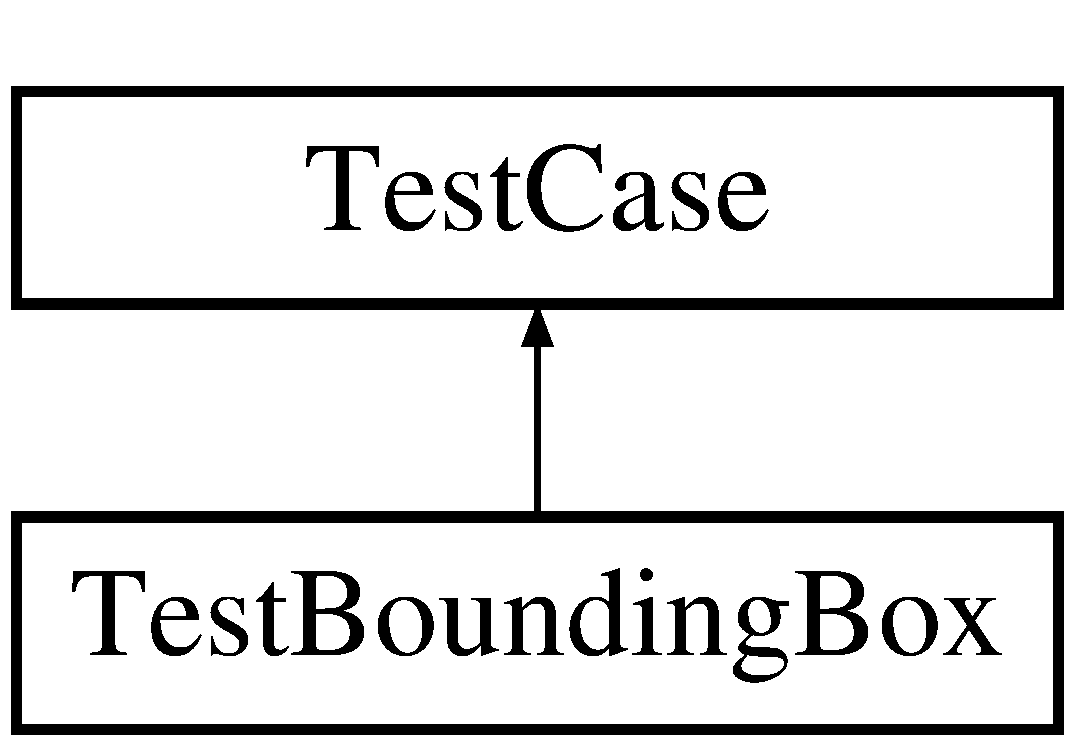
\includegraphics[height=2.000000cm]{classTestBoundingBox}
\end{center}
\end{figure}
\subsection*{Public Member Functions}
\begin{DoxyCompactItemize}
\item 
\mbox{\Hypertarget{classTestBoundingBox_adb12b1e9837925f231153b871a754c70}\label{classTestBoundingBox_adb12b1e9837925f231153b871a754c70}} 
{\bfseries Test\+Bounding\+Box} (std\+::string name)
\item 
\mbox{\Hypertarget{classTestBoundingBox_ac449ddf823b4c456f6ac9f7020540db9}\label{classTestBoundingBox_ac449ddf823b4c456f6ac9f7020540db9}} 
void {\bfseries test\+Overlap} ()
\end{DoxyCompactItemize}


The documentation for this class was generated from the following file\+:\begin{DoxyCompactItemize}
\item 
Collides\+True.\+h\end{DoxyCompactItemize}

\hypertarget{classVector3}{}\section{Vector3 Class Reference}
\label{classVector3}\index{Vector3@{Vector3}}


{\ttfamily \#include $<$Math.\+h$>$}

\subsection*{Public Member Functions}
\begin{DoxyCompactItemize}
\item 
\mbox{\Hypertarget{classVector3_aa2ac7a9dd9ff6523a7decf564d525058}\label{classVector3_aa2ac7a9dd9ff6523a7decf564d525058}} 
{\bfseries Vector3} (const float, const float, const float)
\item 
\mbox{\Hypertarget{classVector3_af327009e11b3169bb2d825e8ea5cbd6b}\label{classVector3_af327009e11b3169bb2d825e8ea5cbd6b}} 
{\bfseries Vector3} (const \hyperlink{classVector3}{Vector3} \&)
\item 
\mbox{\Hypertarget{classVector3_a0e0fe85e0cf7a1bbe8f88b124ba75247}\label{classVector3_a0e0fe85e0cf7a1bbe8f88b124ba75247}} 
const float {\bfseries getX} () const
\item 
\mbox{\Hypertarget{classVector3_af469b793596e9222177f2b19468db175}\label{classVector3_af469b793596e9222177f2b19468db175}} 
const float {\bfseries getY} () const
\item 
\mbox{\Hypertarget{classVector3_afa596479a0e9009955d504554e2a43ce}\label{classVector3_afa596479a0e9009955d504554e2a43ce}} 
const float {\bfseries getZ} () const
\item 
\mbox{\Hypertarget{classVector3_a94f315ca92708d8430bb1ff9fedae0a8}\label{classVector3_a94f315ca92708d8430bb1ff9fedae0a8}} 
const \hyperlink{classVector3}{Vector3} {\bfseries operator+} (const \hyperlink{classVector3}{Vector3} \&) const
\item 
\mbox{\Hypertarget{classVector3_a9d6e8d93fb365ae671053eff9a909fa6}\label{classVector3_a9d6e8d93fb365ae671053eff9a909fa6}} 
const \hyperlink{classVector3}{Vector3} {\bfseries operator$\ast$} (float) const
\end{DoxyCompactItemize}


\subsection{Detailed Description}
A Vector representation somewhat in the style of the I\+B\+M/\+Sony Vectormath library. 

The documentation for this class was generated from the following file\+:\begin{DoxyCompactItemize}
\item 
Math.\+h\end{DoxyCompactItemize}

%--- End generated contents ---

% Index
\backmatter
\newpage
\phantomsection
\clearemptydoublepage
\addcontentsline{toc}{chapter}{Index}
\printindex

\end{document}
